\documentclass{report}

%hyperlinks
\usepackage{hyperref}

%math font
\usepackage{euler}

%set document margin
\usepackage[a4paper, top=.8in, bottom=.4in, left=.75in, right=.75in]{geometry}

%font-related stuff
\usepackage{fontspec}
\usepackage{xltxtra}
\usepackage{xunicode}

%add toc in toc
\usepackage{tocbibind}

%we're going to need images
\usepackage{graphicx}

%set the default font
\setmainfont[ExternalLocation=fonts/]{Ubuntu-R}%
  [Ligatures=TeX,
  BoldFont=Ubuntu-B,
  ItalicFont=Ubuntu-RI,
  BoldItalicFont=Ubuntu-BI]
  
\setmonofont[ExternalLocation=fonts/]{UbuntuMono-R}
  [BoldFont=UbuntuMono-B,
  ItalicFont=UbuntuMono-RI,
  BoldItalicFont=UbuntuMono-BI]

%fix monospace font
\usepackage{listings}
\lstset{columns=fixed, basicstyle=\ttfamily, basewidth=0.5em}
  
%set font
\newfontfamily\secfont[ExternalLocation=fonts/]{Ubuntu-R}
\newfontfamily\titfont[ExternalLocation=fonts/]{Ubuntu-C}

%enable hyperlinks
\usepackage{hyperref}

%make paragraphs nice
\usepackage[parfill]{parskip}

%title formats
\usepackage{titlesec}

\titleformat*{\section}{\secfont\LARGE}
\titleformat*{\subsection}{\secfont\itshape\Large}
\titleformat{\chapter}[display]{\secfont}{\raggedleft\fontsize{60pt}{60pt}\secfont\selectfont\thechapter}{0em}{\raggedleft\fontsize{30pt}{20pt}\secfont\selectfont}

%decrease top spacing of new chapter
\titlespacing*{\chapter}{0pt}{-30pt}{20pt}

%table stuff
\usepackage{tabularx}

%stuff for programming
\usepackage{etoolbox}

%make itemize not suck
\usepackage{enumitem}
\setitemize{noitemsep,topsep=0pt,parsep=0pt,partopsep=0pt}

%appendix functionality
\usepackage{appendix}

\usepackage{polyglossia}
\usepackage{csquotes}

%images
\usepackage{tikz}

%document metadata
\newcommand {\authors} {Authors, Go, Here}
\newcommand {\supervisors} {Your, Supervisors}
\newcommand {\doctitle} {Project Title}
\newcommand {\class} {Class Name (CLSC0D3)}
\newcommand {\contents} {Contents of Document}
\newcommand {\mybibliography} {\addbibresource{references.bib}}

\setdefaultlanguage{dutch}

%ieee bibliography
\usepackage[
backend=biber,
style=alphabetic,
citestyle=authoryear
]{biblatex}

\mybibliography{}

\usepackage{array}
\newcolumntype{P}{>{\normalsize}p{2.5cm}}

\usepackage{ltablex}

\newcommand{\header}[1]{
\fontsize{16pt}{25pt}\titfont\selectfont
        >  #1 
        \vspace{.2cm}
        \hrule
    
    \fontsize{13pt}{12pt}\secfont\selectfont}
\newcommand{\entry}[3]{#1 & \titfont #2 \newline \secfont\normalsize #3 \vspace{.1cm}\\}
\newcommand{\entryShort}[2]{\secfont #1 & \titfont #2 \vspace{.1cm}\\}
\newcommand{\entrySkill}[2]{\titfont #1 & \secfont #2\\}
\newcommand{\experience}[2]{
    \header{#1}
    \begin{tabularx}{\linewidth}{P | X}
        #2
    \end{tabularx}
}

\newcommand{\aboutMe}[1]{
\fontsize{11pt}{12pt}\secfont\selectfont

#1

\vspace{.2cm}}

\newcommand{\skill}[2]{
    \header{#1}
    \begin{tabular}{r >{\normalsize}l}
        #2
    \end{tabular}
}

\newcommand{\contacts}[2]{
    \fontsize{16pt}{25pt}\titfont\selectfont
        \begin{center} #1 \end{center}
    \fontsize{11pt}{12pt}\secfont\selectfont
    \begin{tabularx}{\linewidth}{X X X}
        #2
    \end{tabularx}
}


\begin{document}

% set font to Ubuntu Condensed
\pagestyle{empty}

\titfont

%\begin{tikzpicture}[remember picture,overlay]
%    \begin{pgfonlayer}{foreground}
%    \node[xshift=1in,yshift=-10mm,anchor=north west] at (current page.north west){%
%    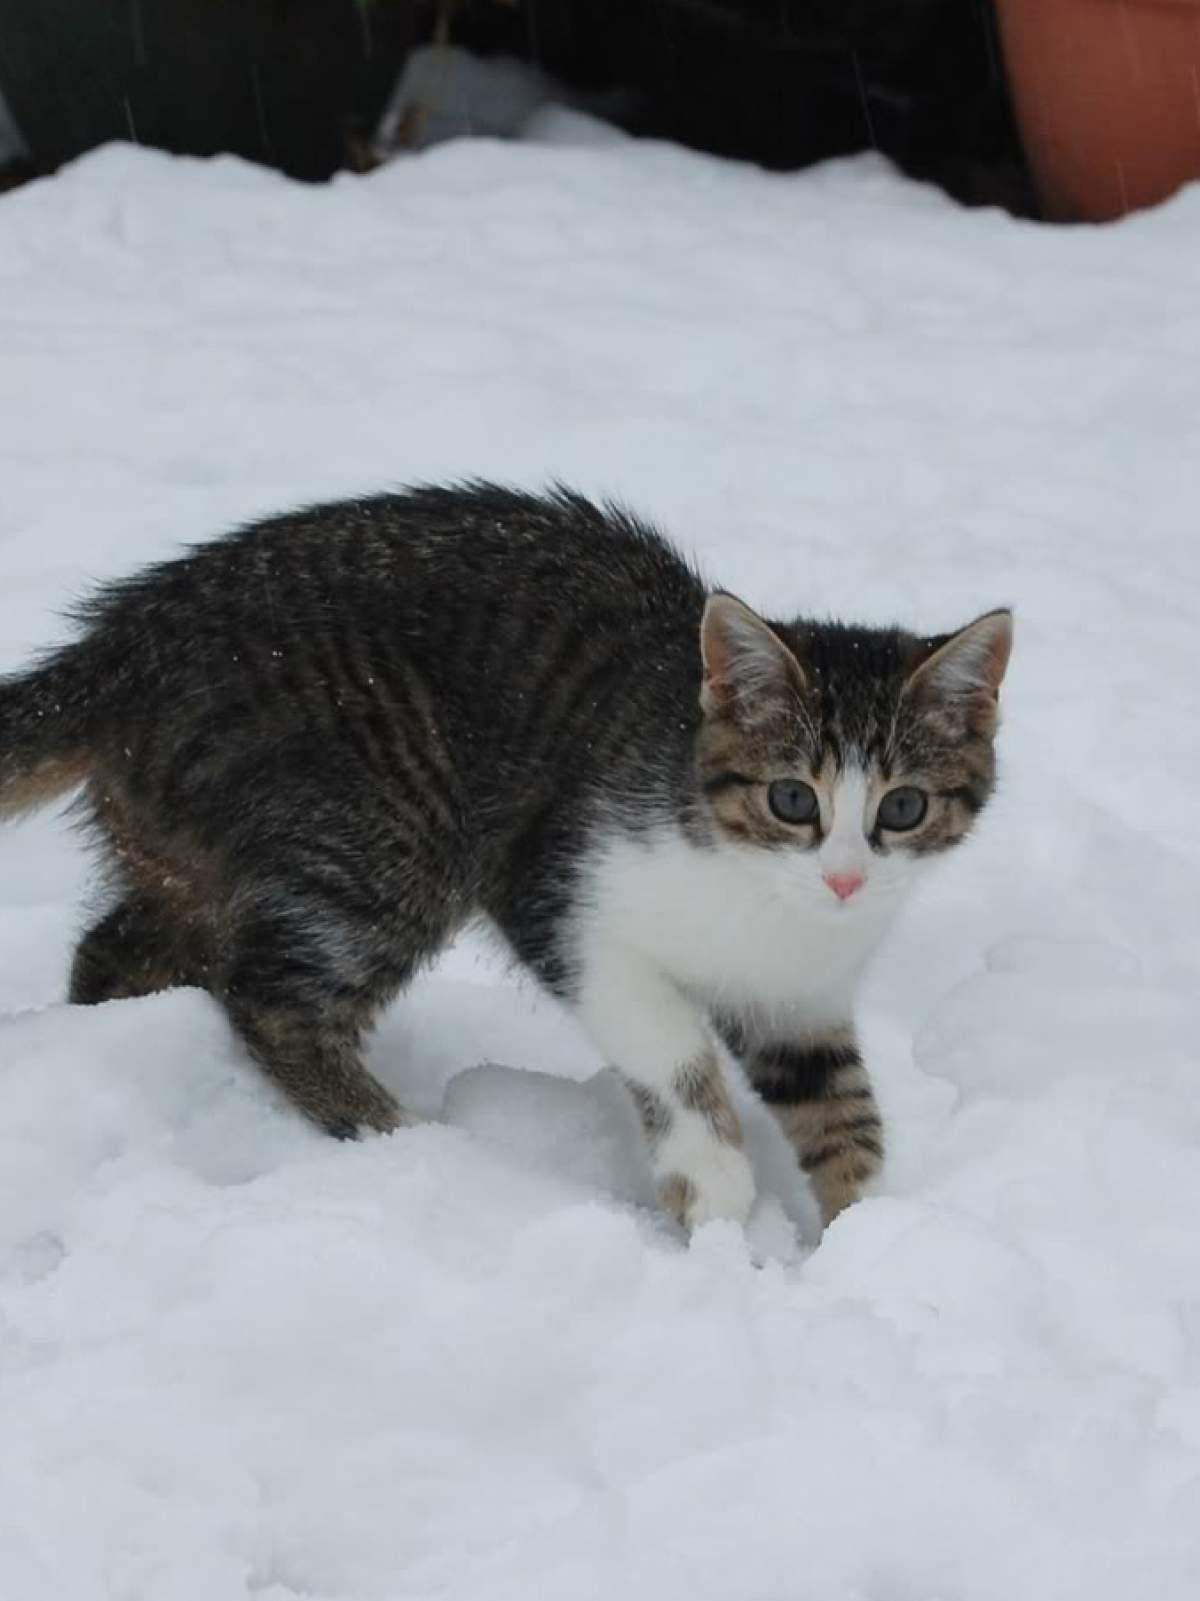
\includegraphics[width=30mm]{photo.jpeg}
%    };
%    \end{pgfonlayer}{foreground}
%\end{tikzpicture}


\begin{flushright}

\fontsize{50pt}{5pt}\selectfont

Rolf Don

\noindent \rule{\textwidth}{1pt} \\ [.28cm]

\fontsize{20pt}{16pt}\titfont\selectfont

Curriculum Vitae

\end{flushright}

\vspace{.5cm}


\secfont

\aboutMe{
I am an inquisitve Computer Engineering student with an affinity for programming and IoT. Throughout the duration of my course, I have found working on projects to automate and improve others' lives very rewarding. I am eager to continue my journey in IT and undertake training and gain experiences to advance my career.
}

\experience{Education}
{
    \entry{2018 - Today}{Student Computer Engineering | Rotterdam University of Applied Sciences}
    {
    I am currently a second year student. In my major, I am working on varied projects including IoT, electrical engineering and programming.
    }
    \entry{2015 - 2017}{Student Systems Administration | ITVitae Learning, Amersfoort}
    {
    I followed a study and working course to start employment as a systems administrator. Throughout my studies, I have learned a lot and worked with many open-source operating systems like Ubuntu Linux, RedHat Linux, Debian Linux and SUSE Linux.
    }
    \entryShort{2014 - 2015}{Student Molecular Science and Technology | TU Delft}
    \entryShort{2013 - 2014}{Student Computer Engineering | TU Delft}
    \entry{2006 - 2013}{VWO NG-NT | Lentiz Groen van Prinstererlyceum, Vlaardingen}
    {
    I took extra classes of Latin and Ancient Greek. I also followed extra English classes for an IB English A Language \& Literature HL certificate.
    }
}

\experience{Employment History}
{
    \entry{2019 - Today}{Teaching Assistant | Rotterdam University of Applied Sciences}
    {
    I help assist teachers teach during class. I also teach extracurricular to help overachieving students challenge themselves.
    }
    \entry{2015 - 2016}{Intern Systems Administration | Fox-IT, Delft}
    {
    I worked on an assignment involving optimizing and documenting Fox's internal JIRA-installation, and gave advice on how to better deploy their software stack in a closed-off network. I also worked on automatic deployment of new machines using Puppet.
    }
    \entry{2014 - 2017}{Volunteer | De Kroepoekfabriek, Vlaardingen}
    {
    I worked at the front of house to control the lights during a concert. I also helped at the bar to work as a service employee serving beverages.
    }
}

\skill{Skills}
{
    \entrySkill{Programming Languages}{Java, C++, Haskell, Kotlin}
    \entrySkill{Operating Systems}{Ubuntu, Debian, RedHat, SUSE, Windows Server}
    \entrySkill{Software}{MySQL, PostgreSQL, Puppet, JIRA, Apache, NGINX}
    \entrySkill{IoT}{AVR, PIC, Arduino}
    \entrySkill{Languages}{English, Dutch, Mandarin (learning)}
}

\vspace{1cm}

\contacts{Contact me}
{
    rolf@pyonium.dev & +31 6 28 62 41 73 & \href{https://www.linkedin.com/in/rolfdon/}{linkedin.com/in/rolfdon/} 
}

\end{document}
